\section{Methods}
\subsection{Data}
We build on dataset that was used in \cite{gkotsis2017characterisation} where they analyze textual content for the root posts in a Subreddit called Suicide Watch\footnote{\url{https://www.reddit.com/r/SuicideWatch/}}. The dataset contains a dump of 53 thousand posts from the suicide watch sub-reddit. 
However the dataset did not contain the threaded conversations for each thread. Reddit is a platform where a user can create a post on a sub-reddit, to which several members of a given sub-reddit can interact with. The array of interactions may range from simple up or down votes or posting at different hierarchy of the thread. This creates a hierarchical threaded structure of posts where the conversations are organized as threads of posts. To understand the deeper nature of these posts,  we crawl Reddit to get the threaded conversations\footnote{The code to crawl reddit for threads can be found at \textit{https://github.com/sagarjoglekar/redditTools}} 

To baseline our work and compare theorized supportive nature of conversations with the broader community, we also crawl other reddit threads. To avoid any bias towards a particular type of subreddit, which have their own culture, we acquire roughly 50 thousand baseline posts which have been popular enough to land on the front page \footnote{The reddit front page algorithm is a combination of popularity and decay in popularity as a function of time. More can be found here \url{https://goo.gl/uVdHjn}}. We crawl the Frontpage posts for 2 weeks accumulating over 50 thousand reddit threads in the process. 

Figure\ref{fig:responseDist} shows the CDF for the number of responses a Root post gets on a thread across the whole dataset. 
\begin{figure}[!htb]
	\centering
	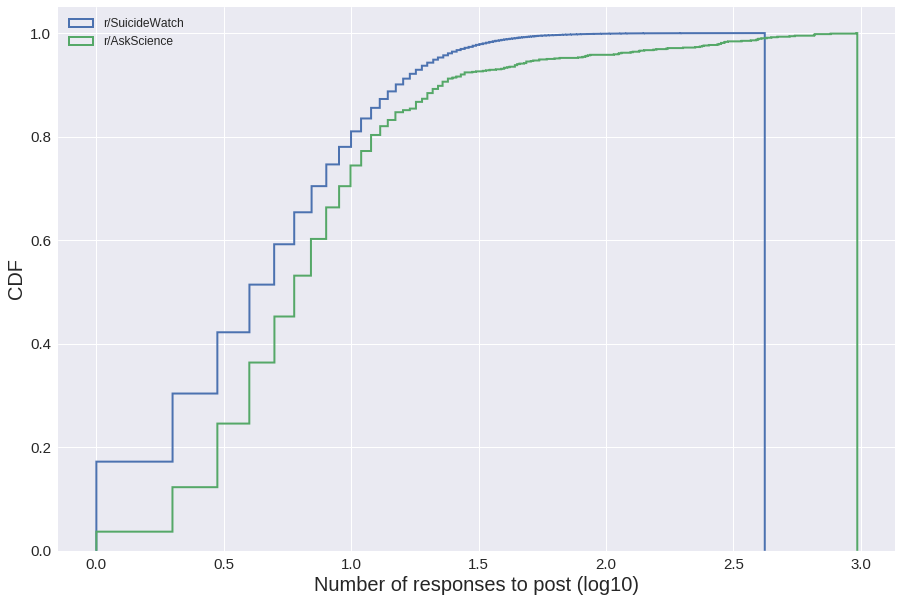
\includegraphics[width=0.5\columnwidth]{Figures/responseDistSW}
	\caption{\textsl{ Distribution of responses per thread on Subreddits r/SuicideWatch and r/AskScience }}
	\label{fig:responseDist}
\end{figure}

Figure \ref{fig:responseDist} shows the CDF for number of comments per thread across the r/SuicideWatch subreddit dataset and the crawled frontpage subreddit. 


\subsection{Abstraction: Networked conversations}

\begin{table}
	\resizebox{0.7\linewidth}{!}{
		\begin{tabular}{l|p{8cm}}
			\textbf{Terminology} & \textbf{stands for}\\
			$RP$   & Root post which begins a new thread on a subreddit \\
			$OP$  & Original poster who posts the Root post for a thread \\
			$BP$   & A Poster who has at-least one symmetric response from the $OP$ after his comment\\
			$AP$   & Asymmetric poster who responds to $OP$ but never gets a response back \\
			$SW$ & The suicide watch Subreddit \\
			$FP$  & Front page of Reddit. \\
			$TD$ & The Donald Subreddit \\
			$AS$ & AskScience subreddit \\
	\end{tabular}}
	\caption{Notations and Terms.}\label{notations}
\end{table}


\label{Sec:Conversations}
To understand the dynamics of supportive conversations, we first need to formalize the abstraction of networked conversations. In case of forum based platforms where users interact in a nested dialogue fashion, and original poster or $OP$ posts a start of a thread. This thread is then open for comments by all the community users. In case of Reddit, such a community is called a Subreddit, which is a moderated collection of users who subscribe to it. These users may post new threads onto the subreddit as far as the post follows the subreddit rules. Enforcement of these rules is the responsibility of the moderators. 

The user who starts a thread is called the Original Poster or $OP$ and the headlining post which the $OP$ begins with is called the Root Post or $RP$. We represent the data using two abstractions. One abstraction is called the \textbf{User Graphs} abstraction. In this method, we represent each thread as a directed graph $G\{V,E,W\}$ where $V$ is the set of all users participating in a particular thread and $E$ are the directed  edges which correspond to interactions between two users $V_i , V_j  \in V$. The weight of each directed edge $E_{ij}$ corresponds to the average Jaccard coefficient calculated on topics covered by posts done by $V_i$ to user $V_J$. 
Formally if $T_i$ is the content of the post posted by $V_i$ and $T_j$ is the content of the post posted by $V_j$ and if $F$ is a topic model trained on the corpus of all texts such that $F(T) \mapsto [t_0 , t_1 \ldots t_n ]$ where $t_k$ is the topic that is present in text $T$, then 
\begin{equation}
	W_{ij} = \frac{F(T_i) \cap F(T_j)}{F(T_i) \cup F(T_j)}
\end{equation}
Where $W_{ij}$ is the edge weight between node $V_i$ and node $V_j$.

The Second abstraction to work with in this paper is the \textbf{Reply Graph} abstraction. We formulate a reply graph $R\{P,E\}$ as a thread of multi-layered posts in a thread in response to the root post $RP$ in the sub-reddit. Each graph $R$ consists of posts $P_i , P_j , i,j \in N$ , where N+1 is the total number of responses in the thread and Edges $E_{ij}$such that and Edge $E_{ij}$ exists $iff$ post $P_i$ was in response to post $P_j$ in the hierarchy of responses. This abstraction works well in modelling the conversational nature of these forums.  For convienece of the reader, we present a couple of example pairs from SW and TheDonald subreddit in Figure \ref{Fig:GraphExamples}
\begin{figure*}[!ht]
	\centering
	% \hspace*{-5mm}
	\subfloat[]{
		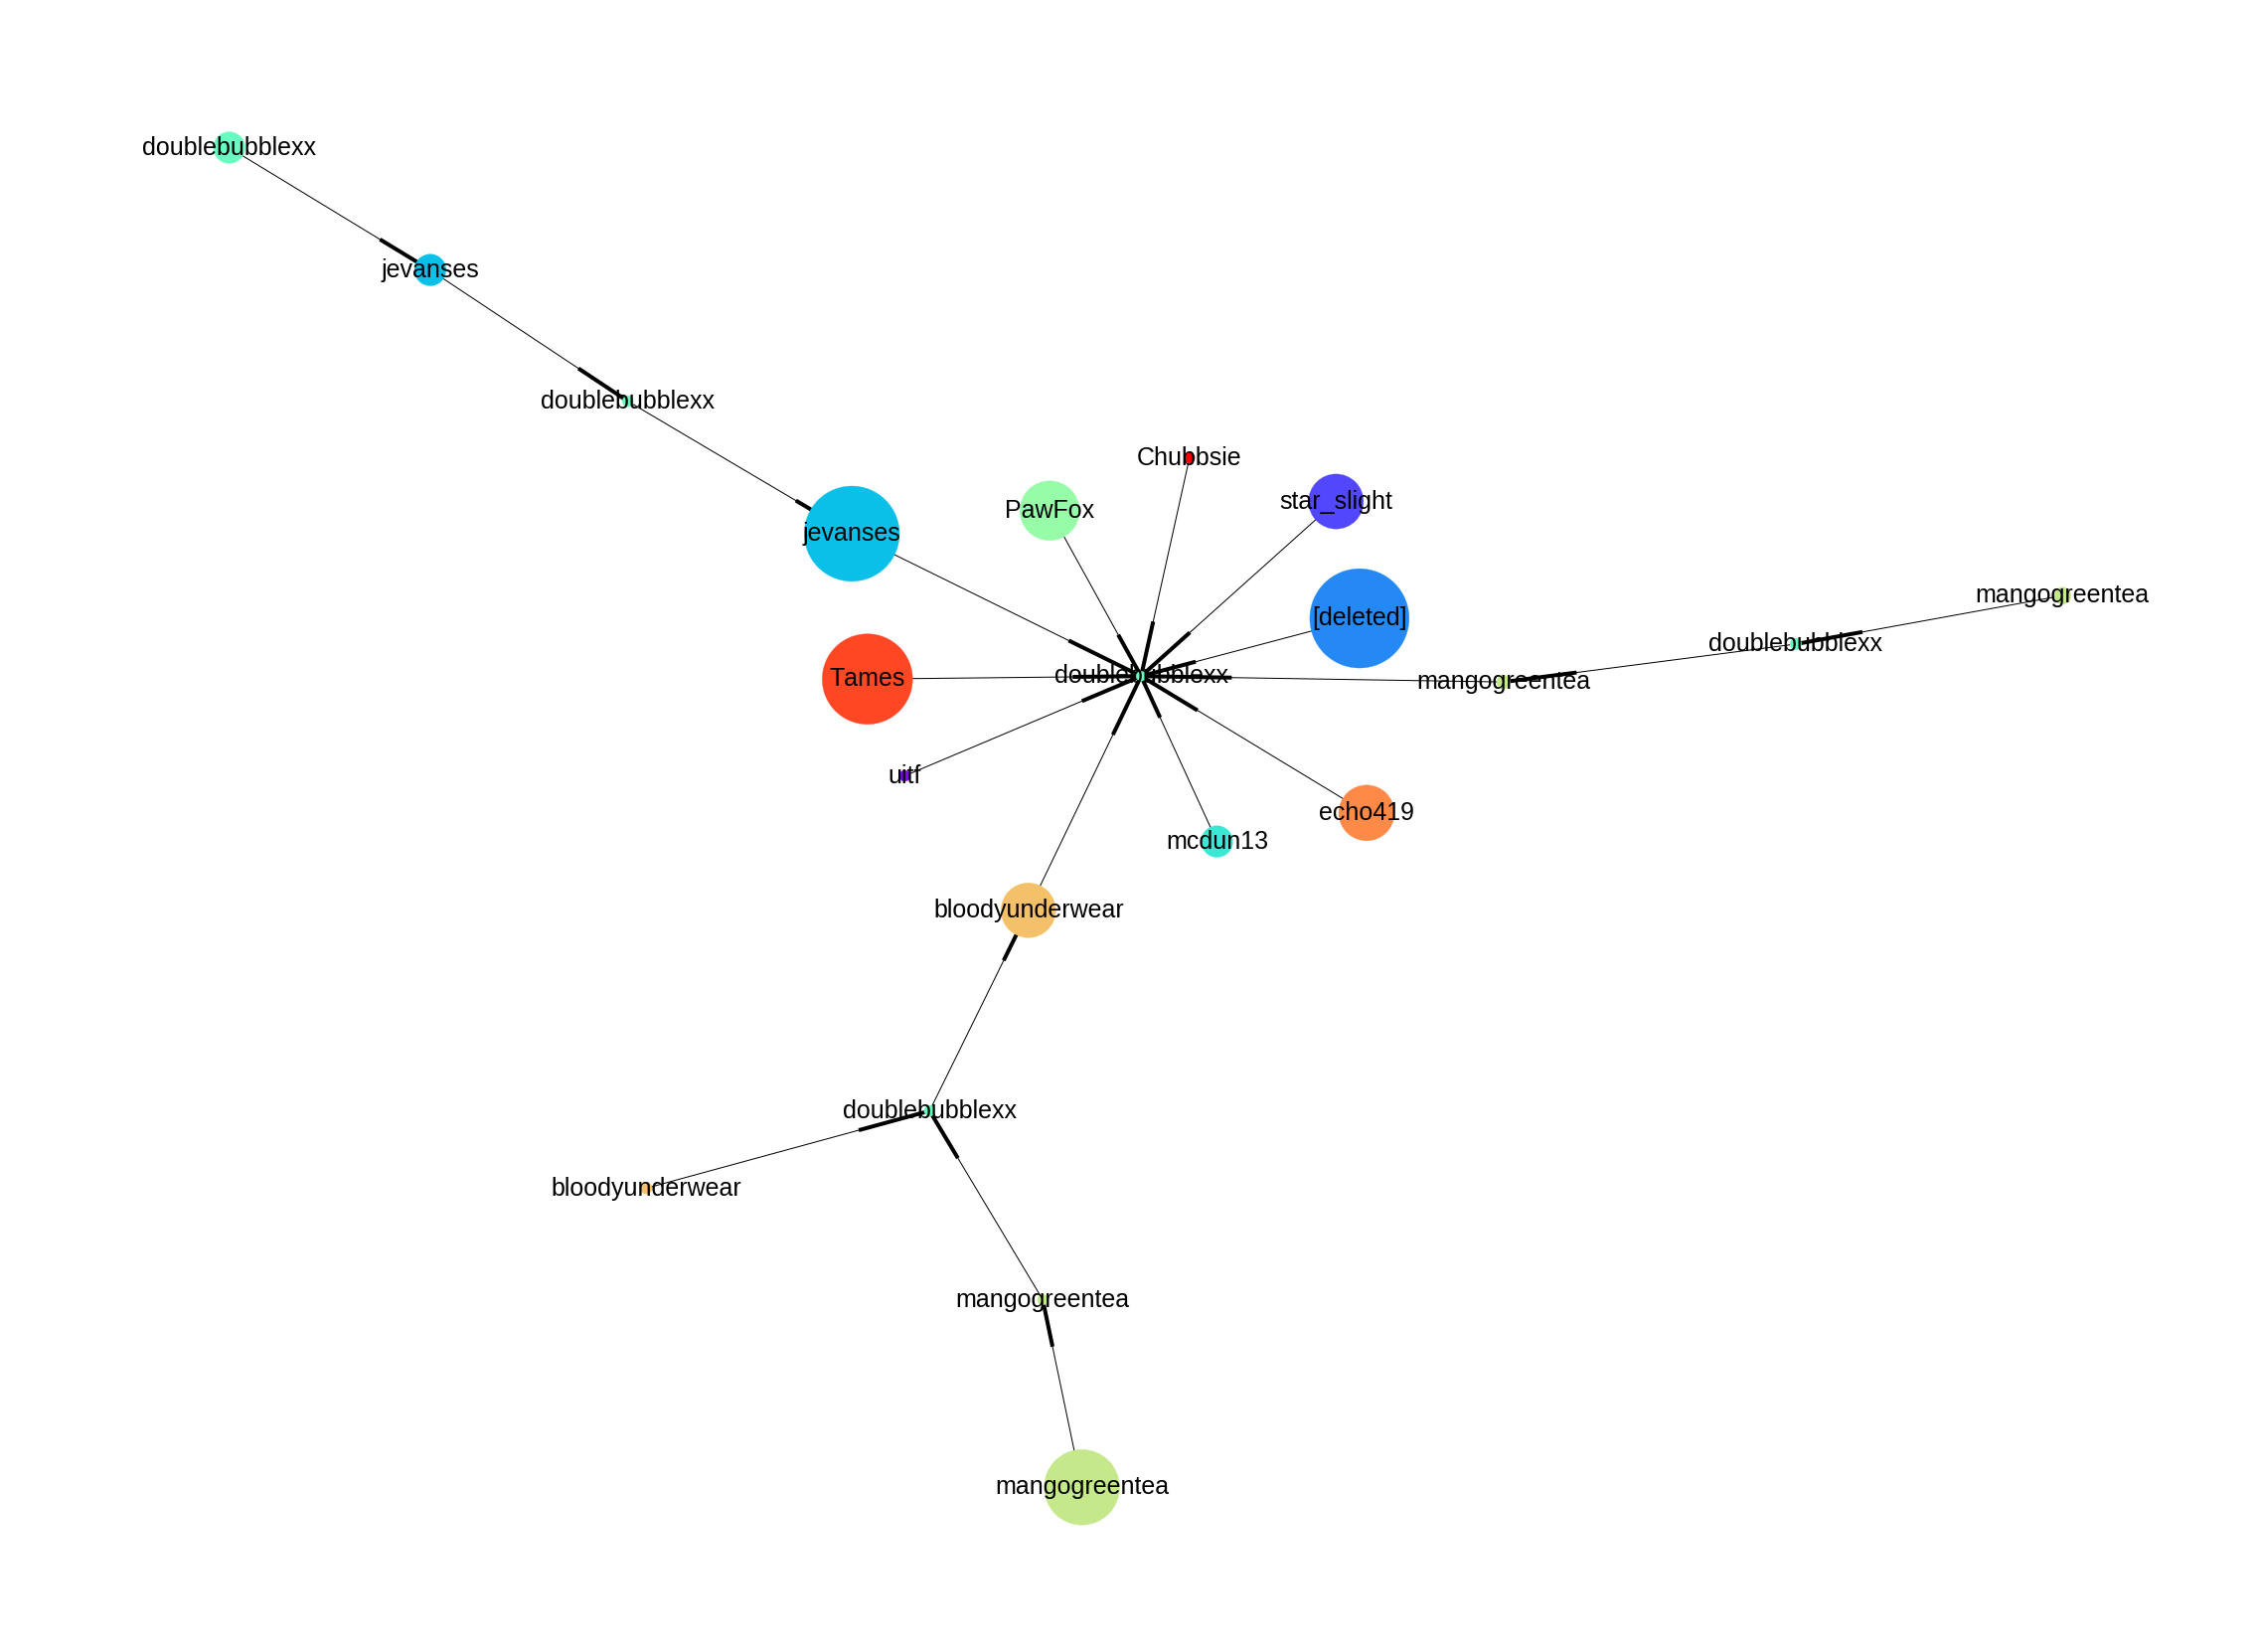
\includegraphics[width=0.45\textwidth, height = 5cm ]{Figures/ReplyGraphSW}
		\label{fig:rGraphSW}
	}
	\subfloat[]{
		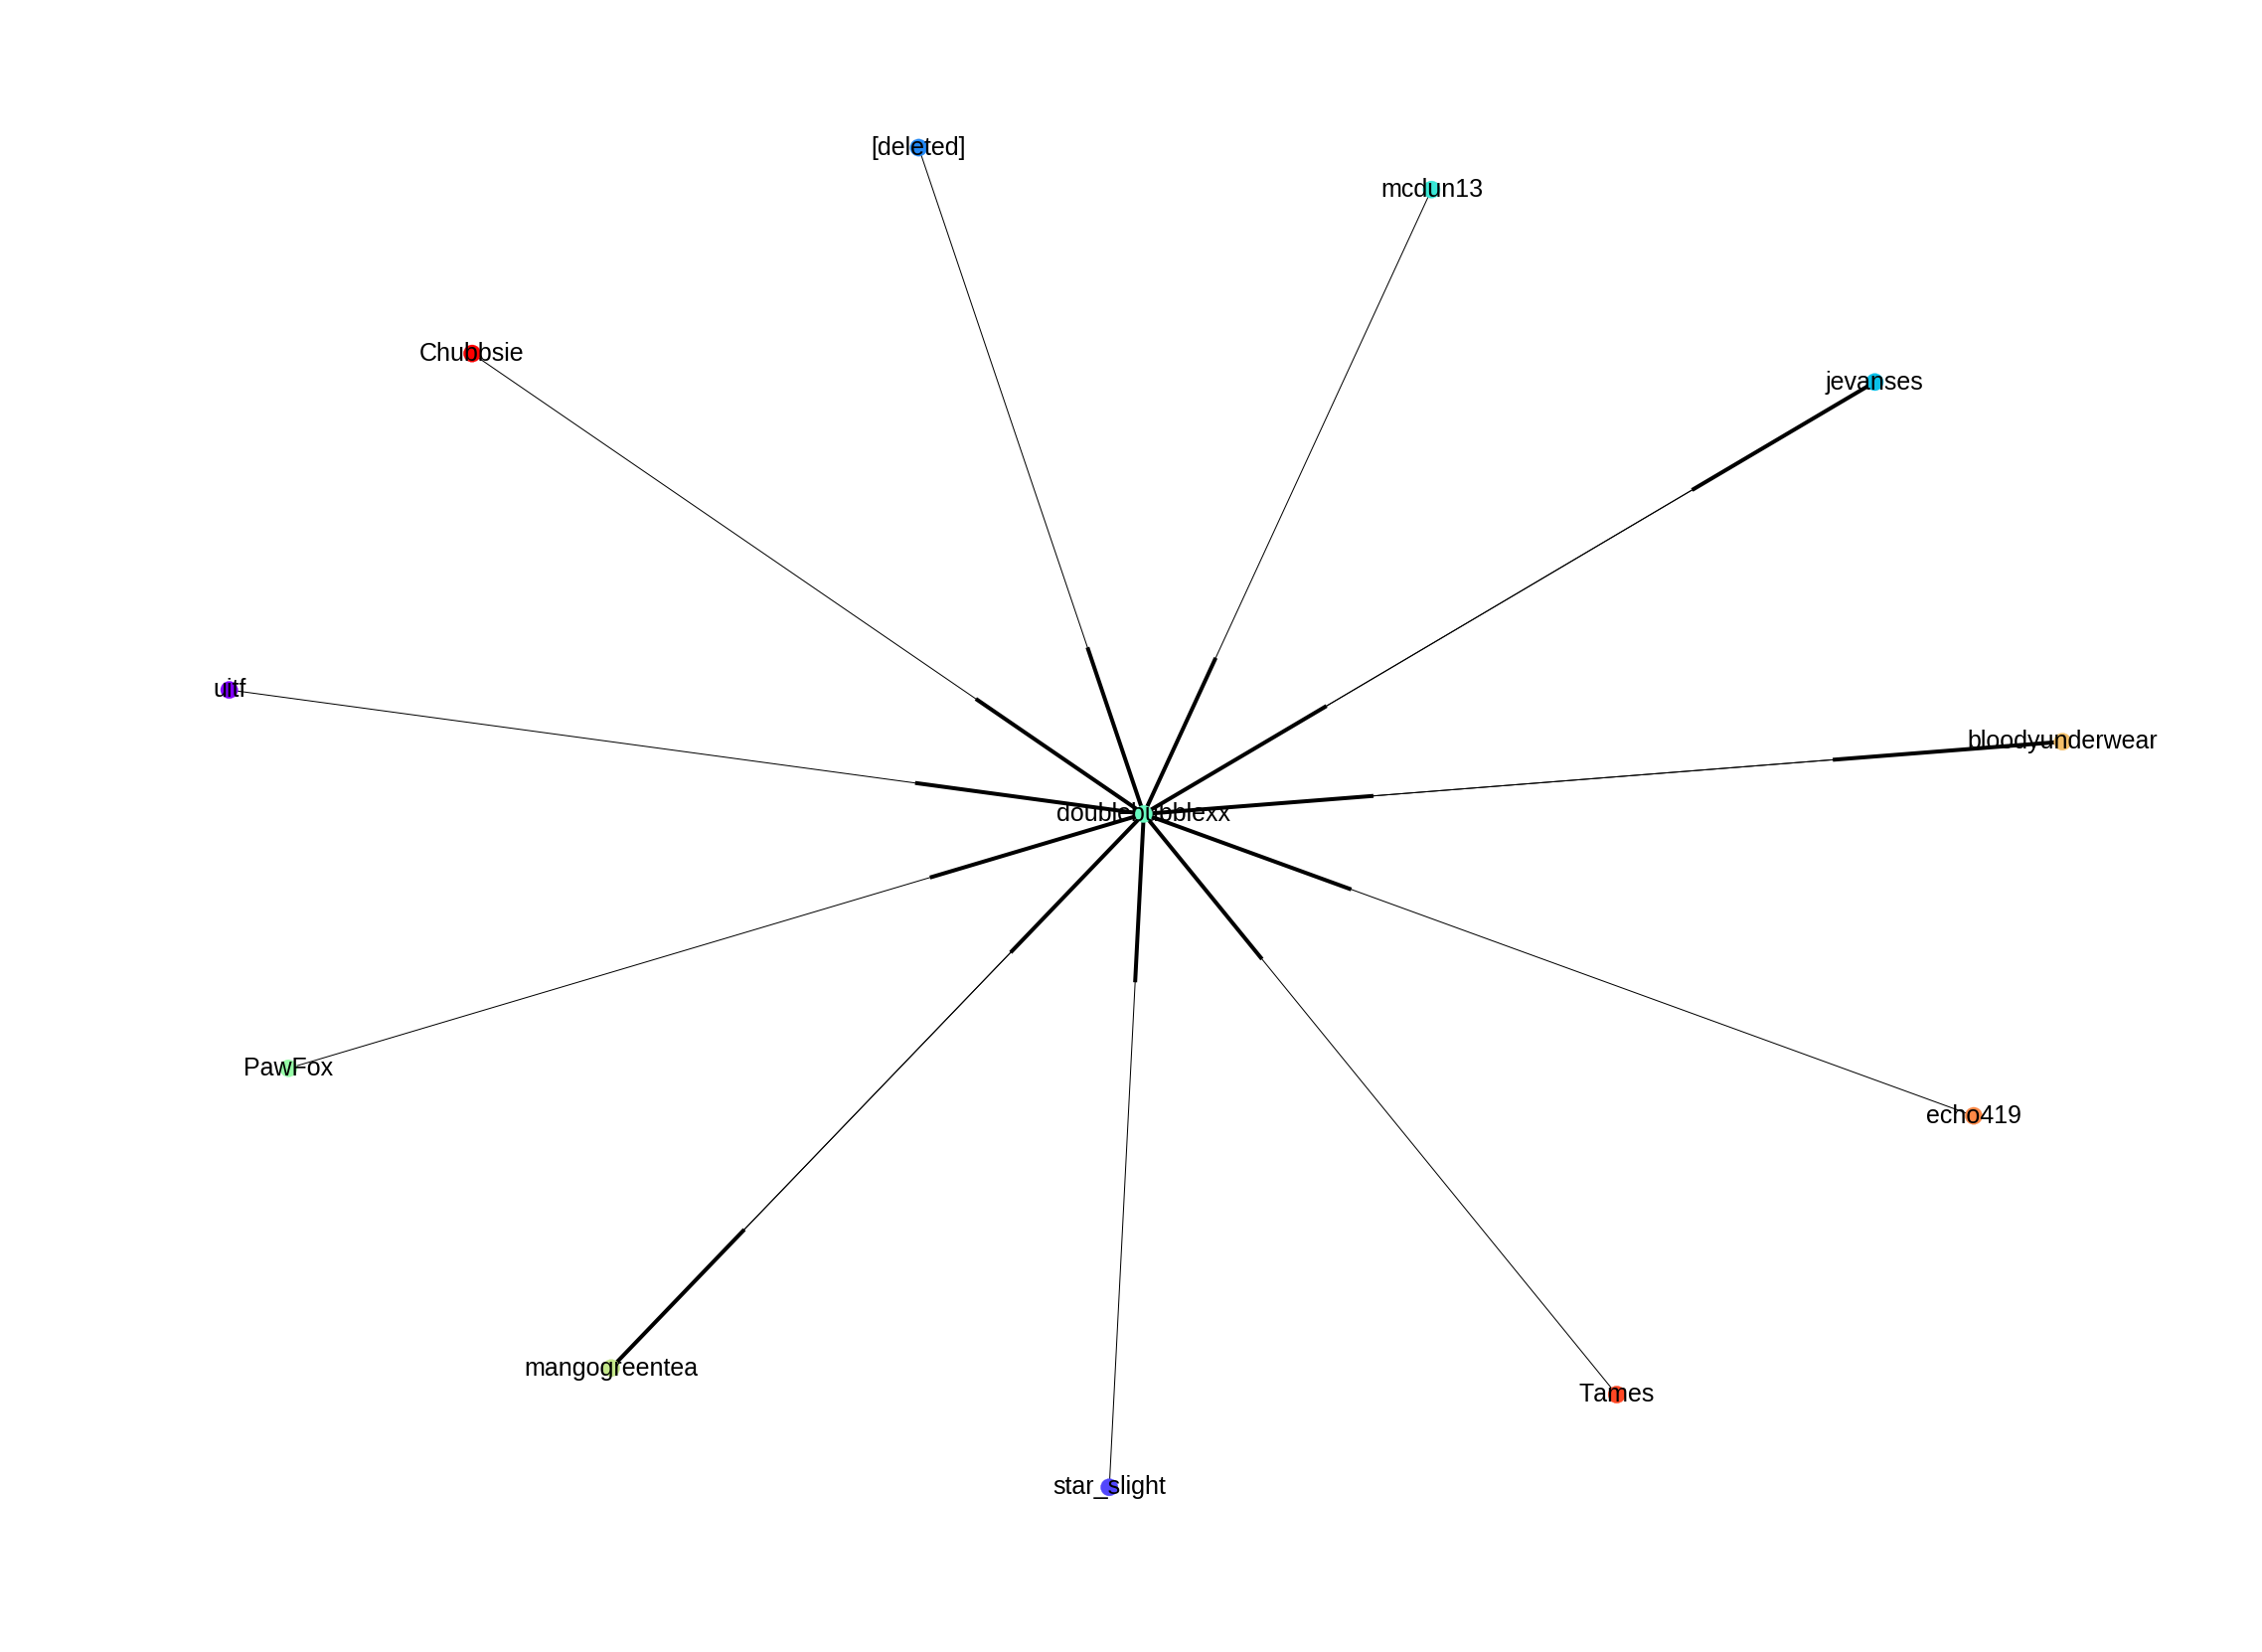
\includegraphics[width=0.45\linewidth, height = 5cm ]{Figures/UserGraphSW}
		\label{fig:uGraphSW}
	}


	\subfloat[]{
		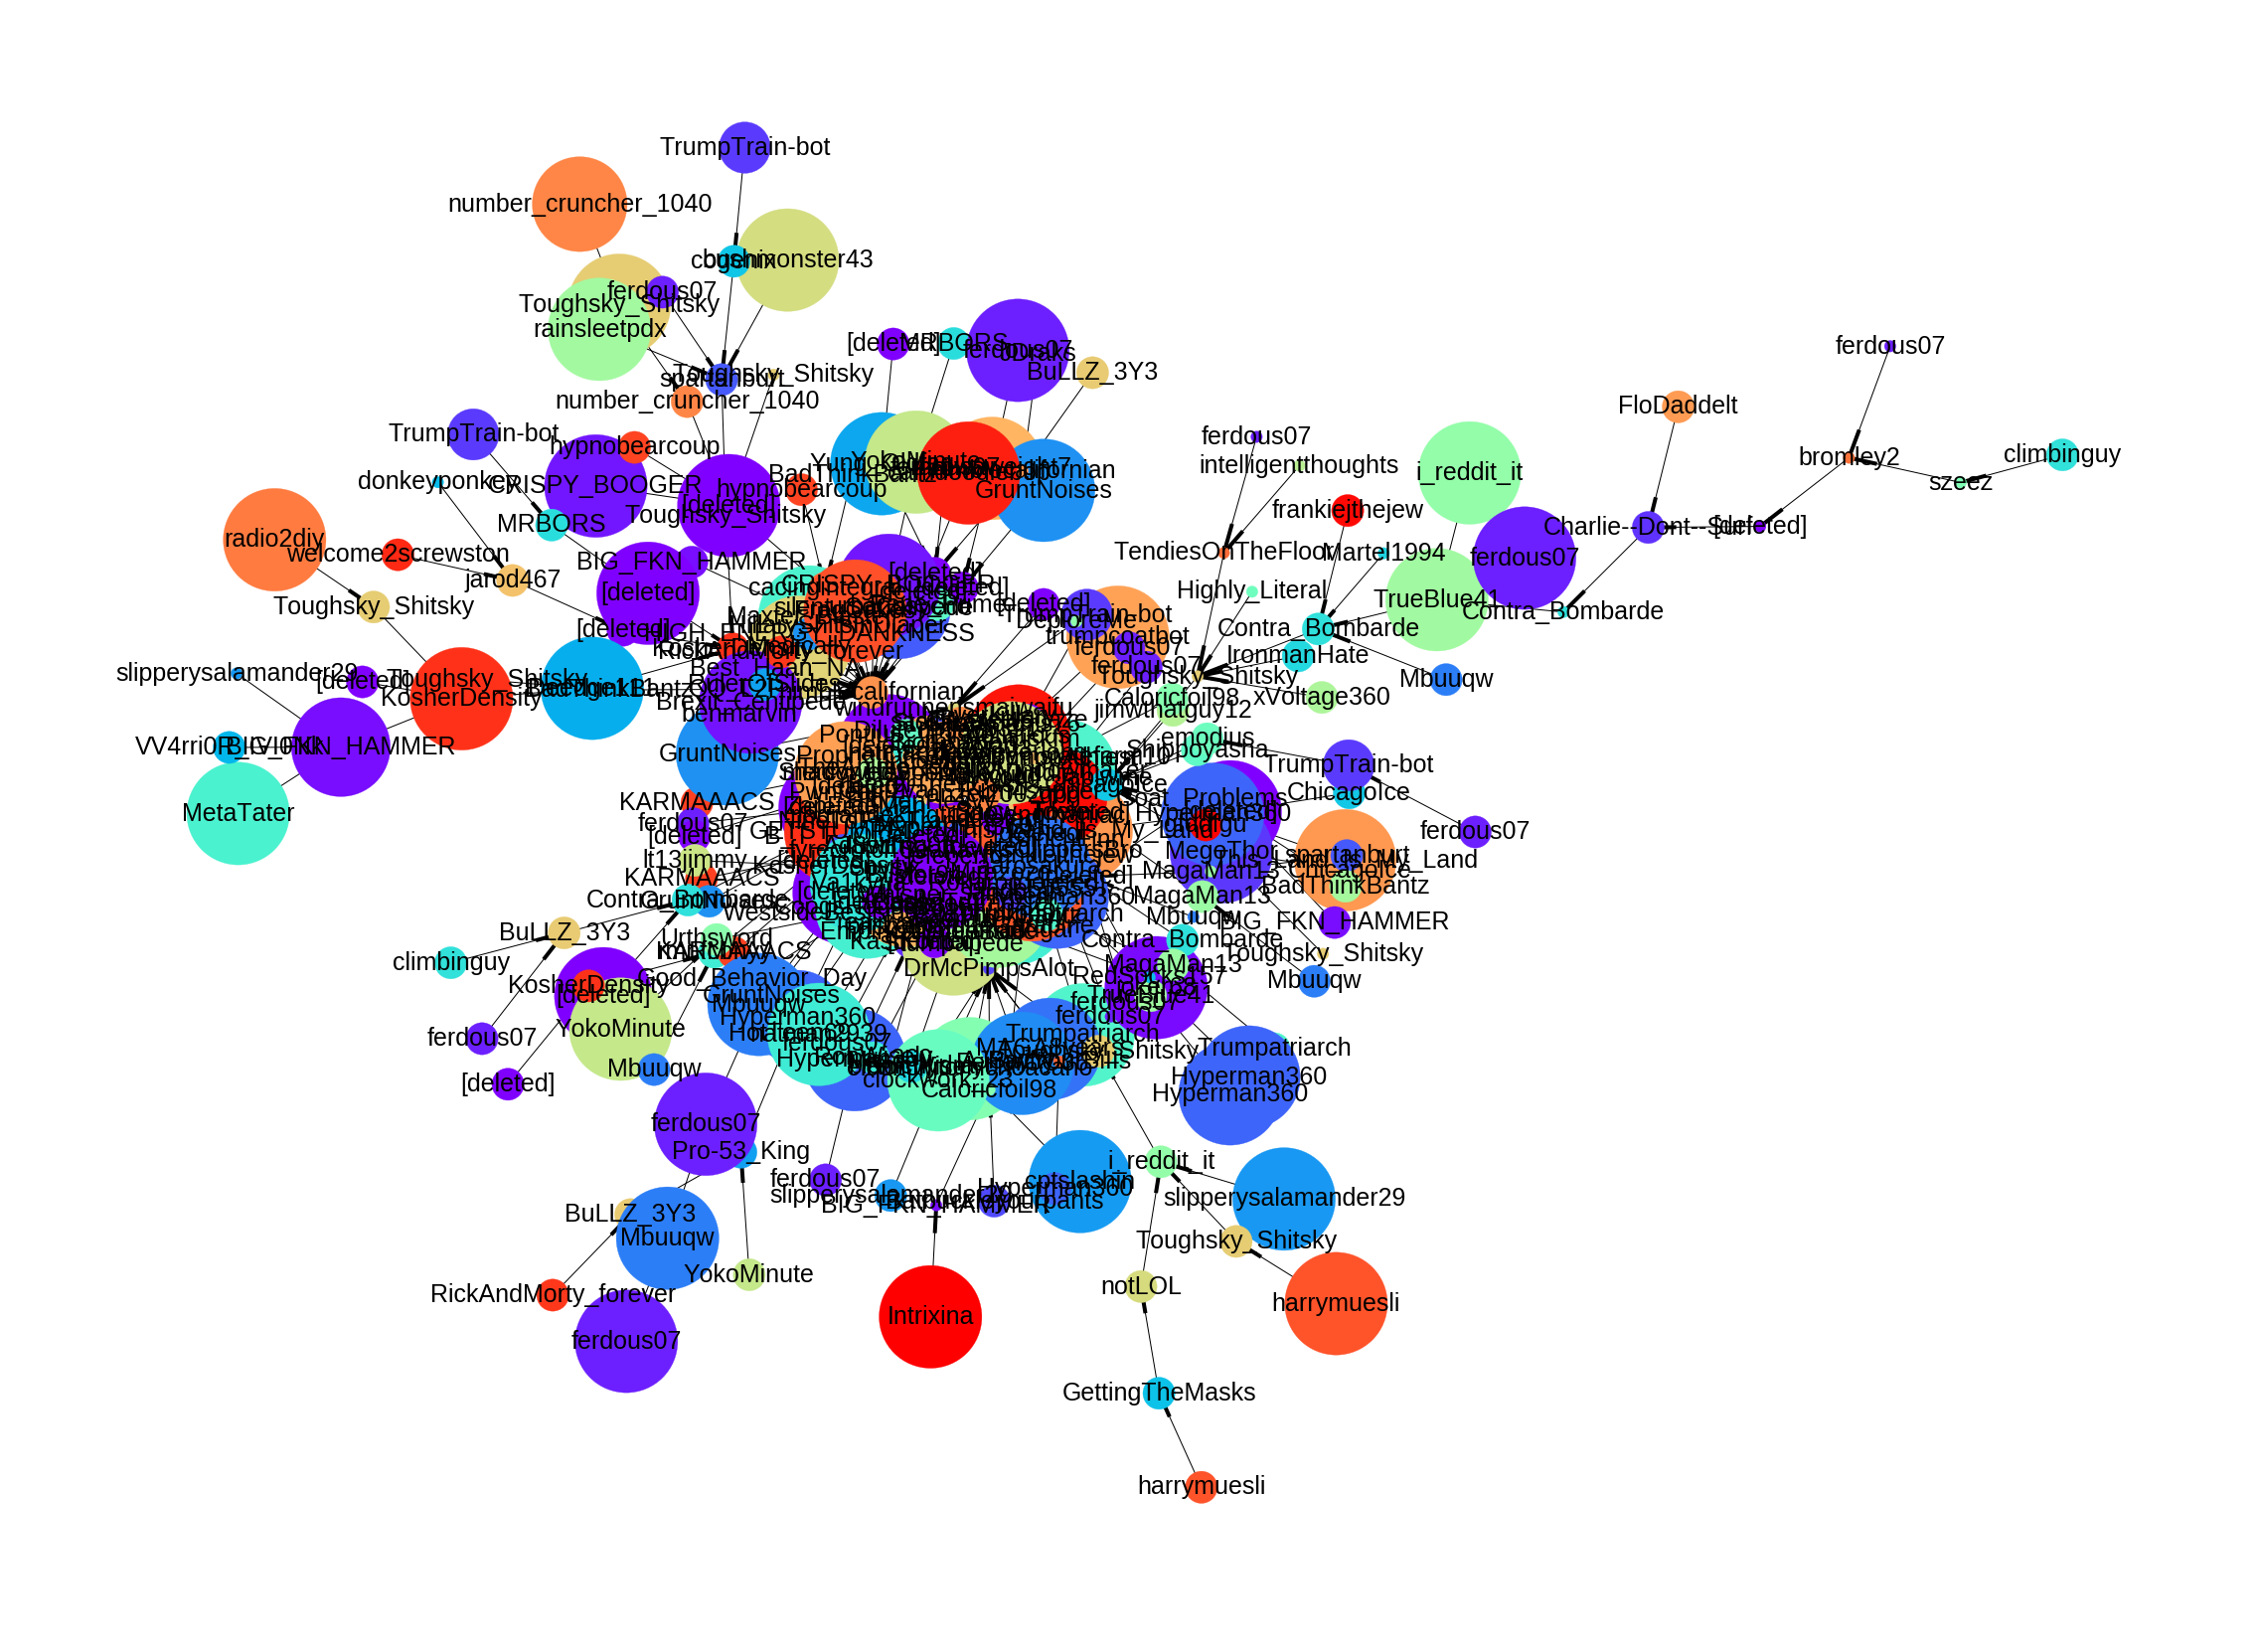
\includegraphics[width=0.45\linewidth, height = 5cm ]{Figures/ReplyGraphTD}
		\label{fig:rGraphTD}
	}
	\subfloat[]{
		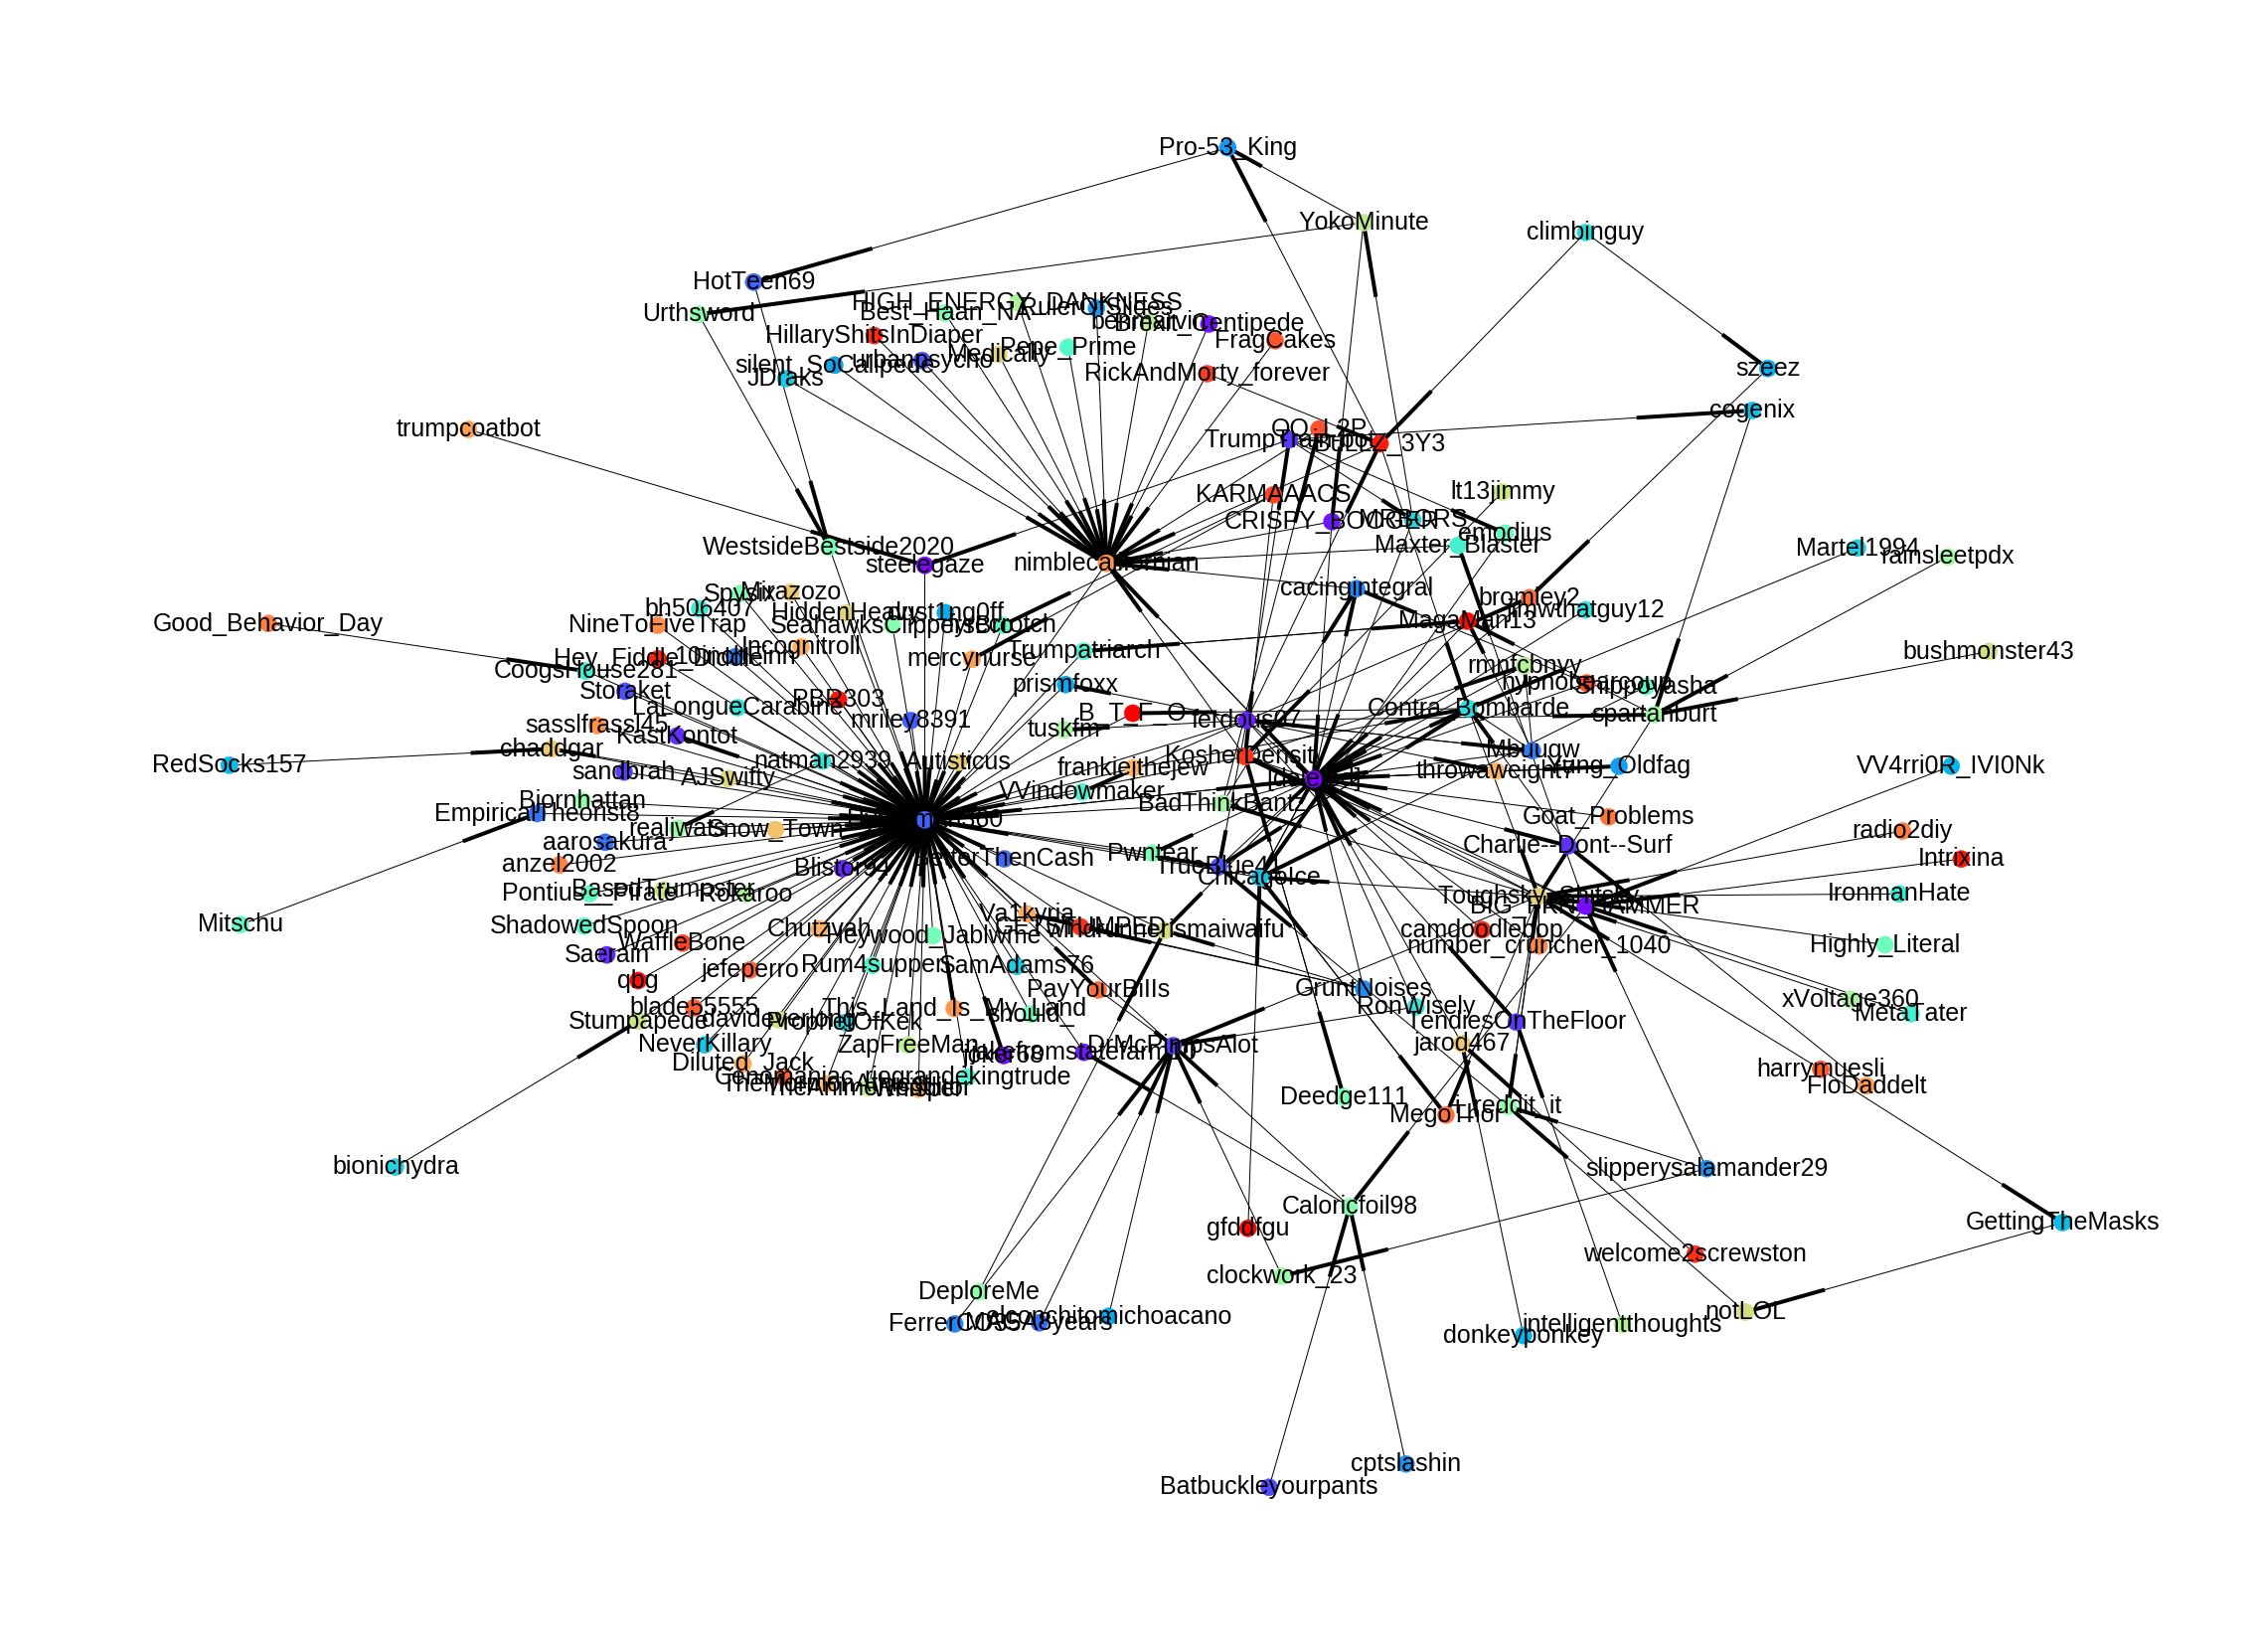
\includegraphics[width=0.45\linewidth, height = 5cm ]{Figures/UserGraphTD}
		\label{fig:uGraphTD}
	}
	\caption{ Example UserGraphs and their corresponding Reply graphs, Figure \ref{fig:uGraphSW} shows a random thread from the SW sub-reddit and \ref{fig:rGraphSW} shows the corresponding reply graph that arises from the response structure of the same thread. In comparison we have Usergraph Fig \ref{fig:uGraphTD} and its corresponding reply graph Fig \ref{fig:rGraphTD} from the subreddit r/TheDonald }
	\label{Fig:GraphExamples}
\end{figure*}

\subsection{Motif Extraction}
To understand relation of local structure in conversations with its nature, we compare the quantity called \textsl{motif occurrence ratio}. After calculating motif census across the dataset\cite{Batagelj2001}, we select progressive subsets of graphs from both datasets with nodes $n \in \{10 , 12 , 15 , 18 , 20 , 22 , 25 , 28 , 30\}$. For each of these node values we get a subset of graphs with those specific number of nodes, from Suicide watch and baseline frontpage, lets call then $\Gamma_{SW}$ and $\Gamma_{BL}$. Let us assume that for a given value of $n$ , $\Gamma_{SW}$ has $K_{SW}$ graphs and $\Gamma_{BL}$ has $K_{BL}$ graphs. We then count for a given motif, number of occurrences in $\Gamma_{SW}$ and $\Gamma_{BL}$ where the graph had at-least one instance of that motif. Let us call the total number of graphs in $\Gamma_{BL}$ with a given motif as $\gamma_{BL}$ and $\gamma_{SW}$ likewise for the $\Gamma_{SW}$ graphs. 
We then define the motif occurrence ratio as the fraction values for $\frac{\gamma_{BL}}{K_{BL}}$ and $\frac{\gamma_{SW}}{K_{SW}}$ for all the 16 motifs across all the chosen values of $n$. 